\documentclass[../MasterThesis.tex]{subfiles}
\graphicspath{ {./assets/images/} }


%----------------------------------------------------------------------------
%----------------------------------------------------------------------------

\begin{document}
	
	
	
%
%
%
%
%=======================================================================================================
%
%
%
%
%=======================================================================================================
% CHAPTER: DESIGN AND IMPLEMENTATION
%=======================================================================================================
\newpage
\section{Design and Implementation} \label{section:designandimplementation}







%-------------------------------------------------------------------------------------------------------
\subsection{Architecture Design} \label{subsection:architecturedesign}
% Describe the overall architecture of the system.

%Provide an overview of the system architecture and design. This could include high-level diagrams, such as system flowcharts or architecture diagrams, to illustrate the structure of the software.
%Introduce the existing codebase and its components. Briefly describe the major modules or sections of the code.
%Explain the design decisions made during the development process. Discuss the rationale behind the chosen architecture, programming languages, and frameworks.
%Present any relevant design patterns or paradigms applied in the codebase.
%Provide a detailed description of how the existing code works. This involves explaining the functionality of key modules or sections, the flow of data, and how different components interact.
%If applicable, discuss any algorithms or data structures implemented in the codebase.
%Highlight any challenges or considerations encountered during the implementation phase and how they were addressed.
%Include code snippets, illustrations, or diagrams to enhance the understanding of your codebase.

TODO: Short overview/introduction of architecture and explain structure of this section?





The connection from the Python backend to the Melt framework can use Melt's capabilities for video editing, processing, transcoding, rendering or playback. The system includes real-time communication via WebRTC, where Melt is involved in handling and manipulating video content.














%-------------------------------------------------------------------------------------------------------
\subsection{Accurate Video} \label{subsection:accuratevideo}
% Describe the frontend


The frontend uses Node.js as its runtime environment. Node.js enables the execution of JavaScript code outside of a web browser.~\cite{nodejs, RM_Frontend, ap3_docs}

To manage project dependencies and packages, either Yarn or npm (Node Package Manager) is used. These package managers allow developers to install, update, and manage libraries and tools used in the project.~\cite{RM_Frontend, npmyarn}


\begin{figure}[H]
	\centering
	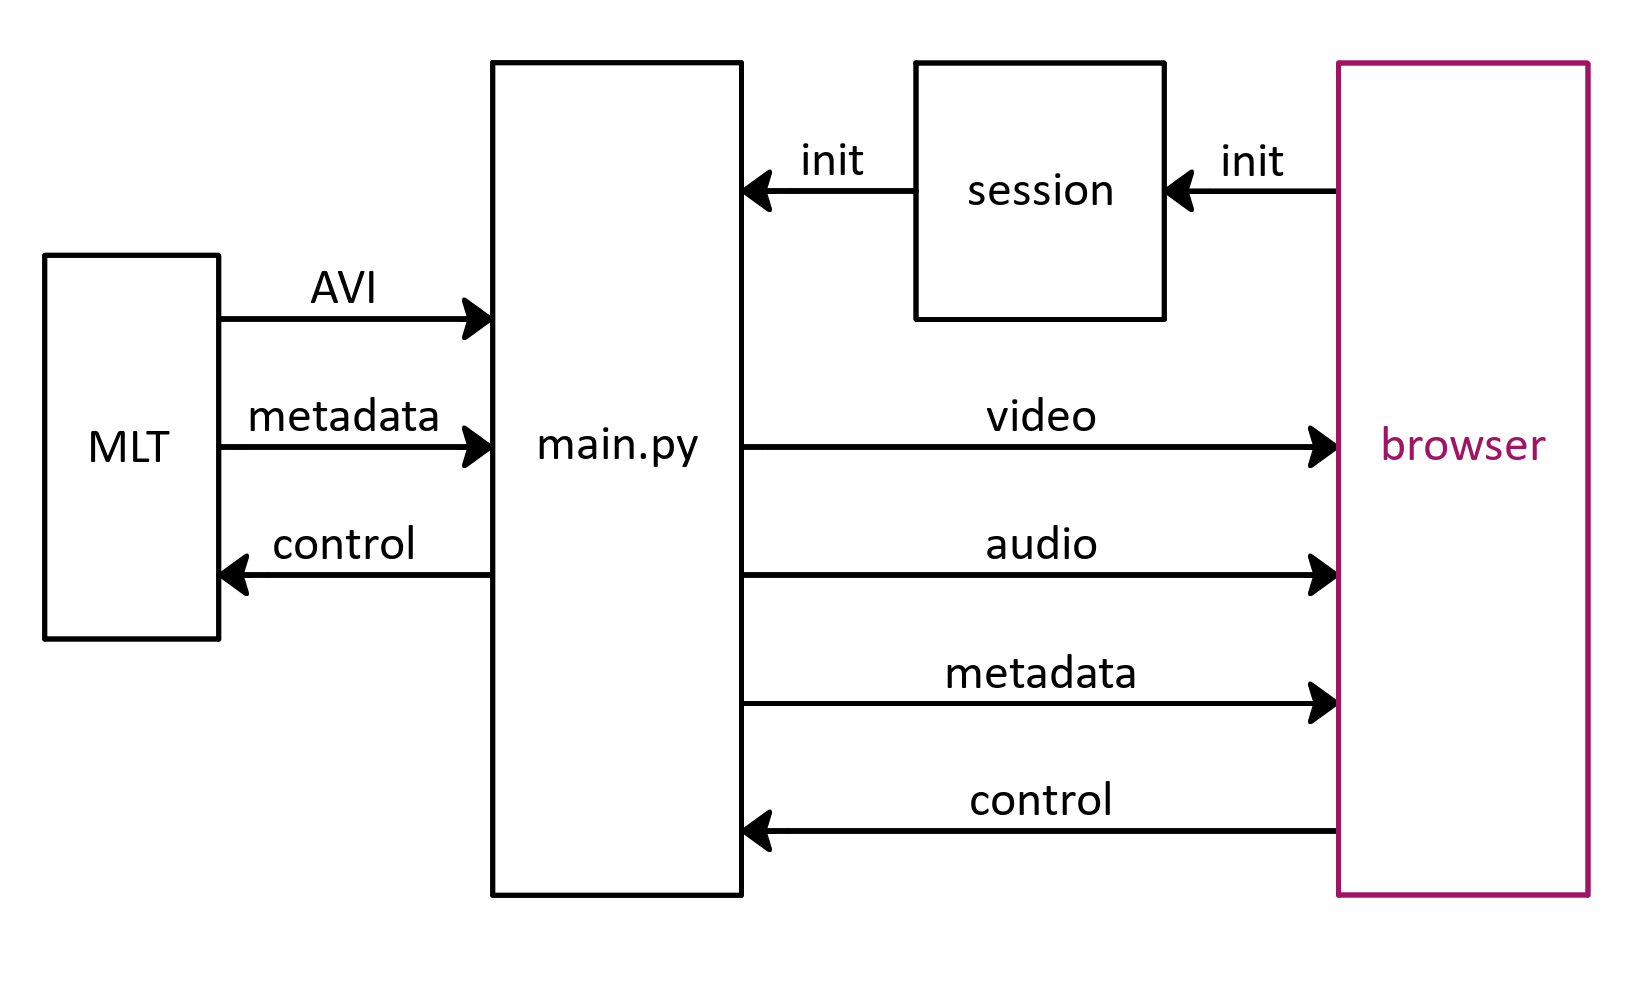
\includegraphics[width=0.5\textwidth]{IM_FE.png}
	\caption{Accurate Video in the system architecture}
\end{figure}













%-------------------------------------------------------------------------------------------------------
\subsection{JIT-WebRTC} \label{subsection:jit-webrtc}
% Describe the backend

The following description of the system is based on the code base and the information from the \texttt{README} file~\cite{RM_Backend}.

JIT-WebRTC is a live transcoder with a WebRTC output. As described in Section~\ref{subsection:technicalbackground}, transcoding is the conversion of one digital data format into another.~\cite{transcoding}

%# jit-webrtc
%
%Live Transcoder with WebRTC output
%

The backend consists of three components that will be described in the following:
\begin{itemize}
	\item Melt
	\item \texttt{main.py}
	\item Session service
\end{itemize}

The system's frontend was described in Section \ref{subsection:accuratevideo}

\begin{figure}[H]
	\centering
	
\includegraphics[width=0.8\textwidth]{IM3.png}
	\caption[System architecture]{Architecture of the system that consits out of four parts.}
\end{figure}

%## Design 
%
%The system consists of four "moving parts": three on the backend (`melt`, `main.py` and `session-service`)
%and one on the frontend (website with a JavaScript/WebRTC client).
%
%```
%                  +---------+      +---------+      +---------+
%                  |         | init |         | init |         |
%                  |         |<-----| session |<-----|         |
%+------+   AVI    |         |      |         |      |         |
%|      |--------->|         |      +---------+      |         |
%|      | metadata |         |         video         |         |
%| melt |--------->| main.py |---------------------->| browser |
%|      | control  |         |         audio         |         |
%|      |<---------|         |---------------------->|         |
%+------+          |         |        metadata       |         |
%                  |         |---------------------->|         |
%                  |         |        control        |         |
%                  |         |<----------------------|         |
%                  +---------+                       +---------+
%```
%


\newpage
%---------------------------------
\subsubsection{Melt}

The Melt framework (MLT/Melt) is a multimedia framework as a command-line (CLI) tool that can be used for video editing and playback. It provides a set of tools, libraries, and services for handling multimedia content, including video and audio.~\cite{melt} 


A variety of tasks can be performed with Melt, including the application of filters on audio or video files, and converting data between different formats. 


%In conclusion, the Melt framework is a valuable tool for anyone who works with data. Its intuitive interface and powerful features make it a versatile and indispensable asset in the data toolbox.

%References:

%Melt Documentation. Available online: [Insert link to Melt documentation here]
%Smith, J. (2020). Getting Started with Data Analysis Using Melt. O'Reilly Media.

% TODO: List and compare different filters and their results


\newpage
%-------------------------------------------------------------------------------------------------------
\subsection{Melt Filter} \label{subsection:meltfilter}


Use of \texttt{avfilter.colorchannelmixer}:

\url{https://www.mltframework.org/plugins/FilterAvfilter-colorchannelmixer/}

\texttt{title: colorchannelmixer \newline
	media types: Video \newline
	description: Adjust colors by mixing color channels.}

Execution of \texttt{melt https://s3.eu-central-1.amazonaws.com/accurate-player\--demo-assets/timecode/sintel-2048-timecode-stereo.mp4 \\ -filter avfilter.colorbalance av.rs=1 av.gm=1 av.bh=1}:


\begin{minipage}{0.5\textwidth}
	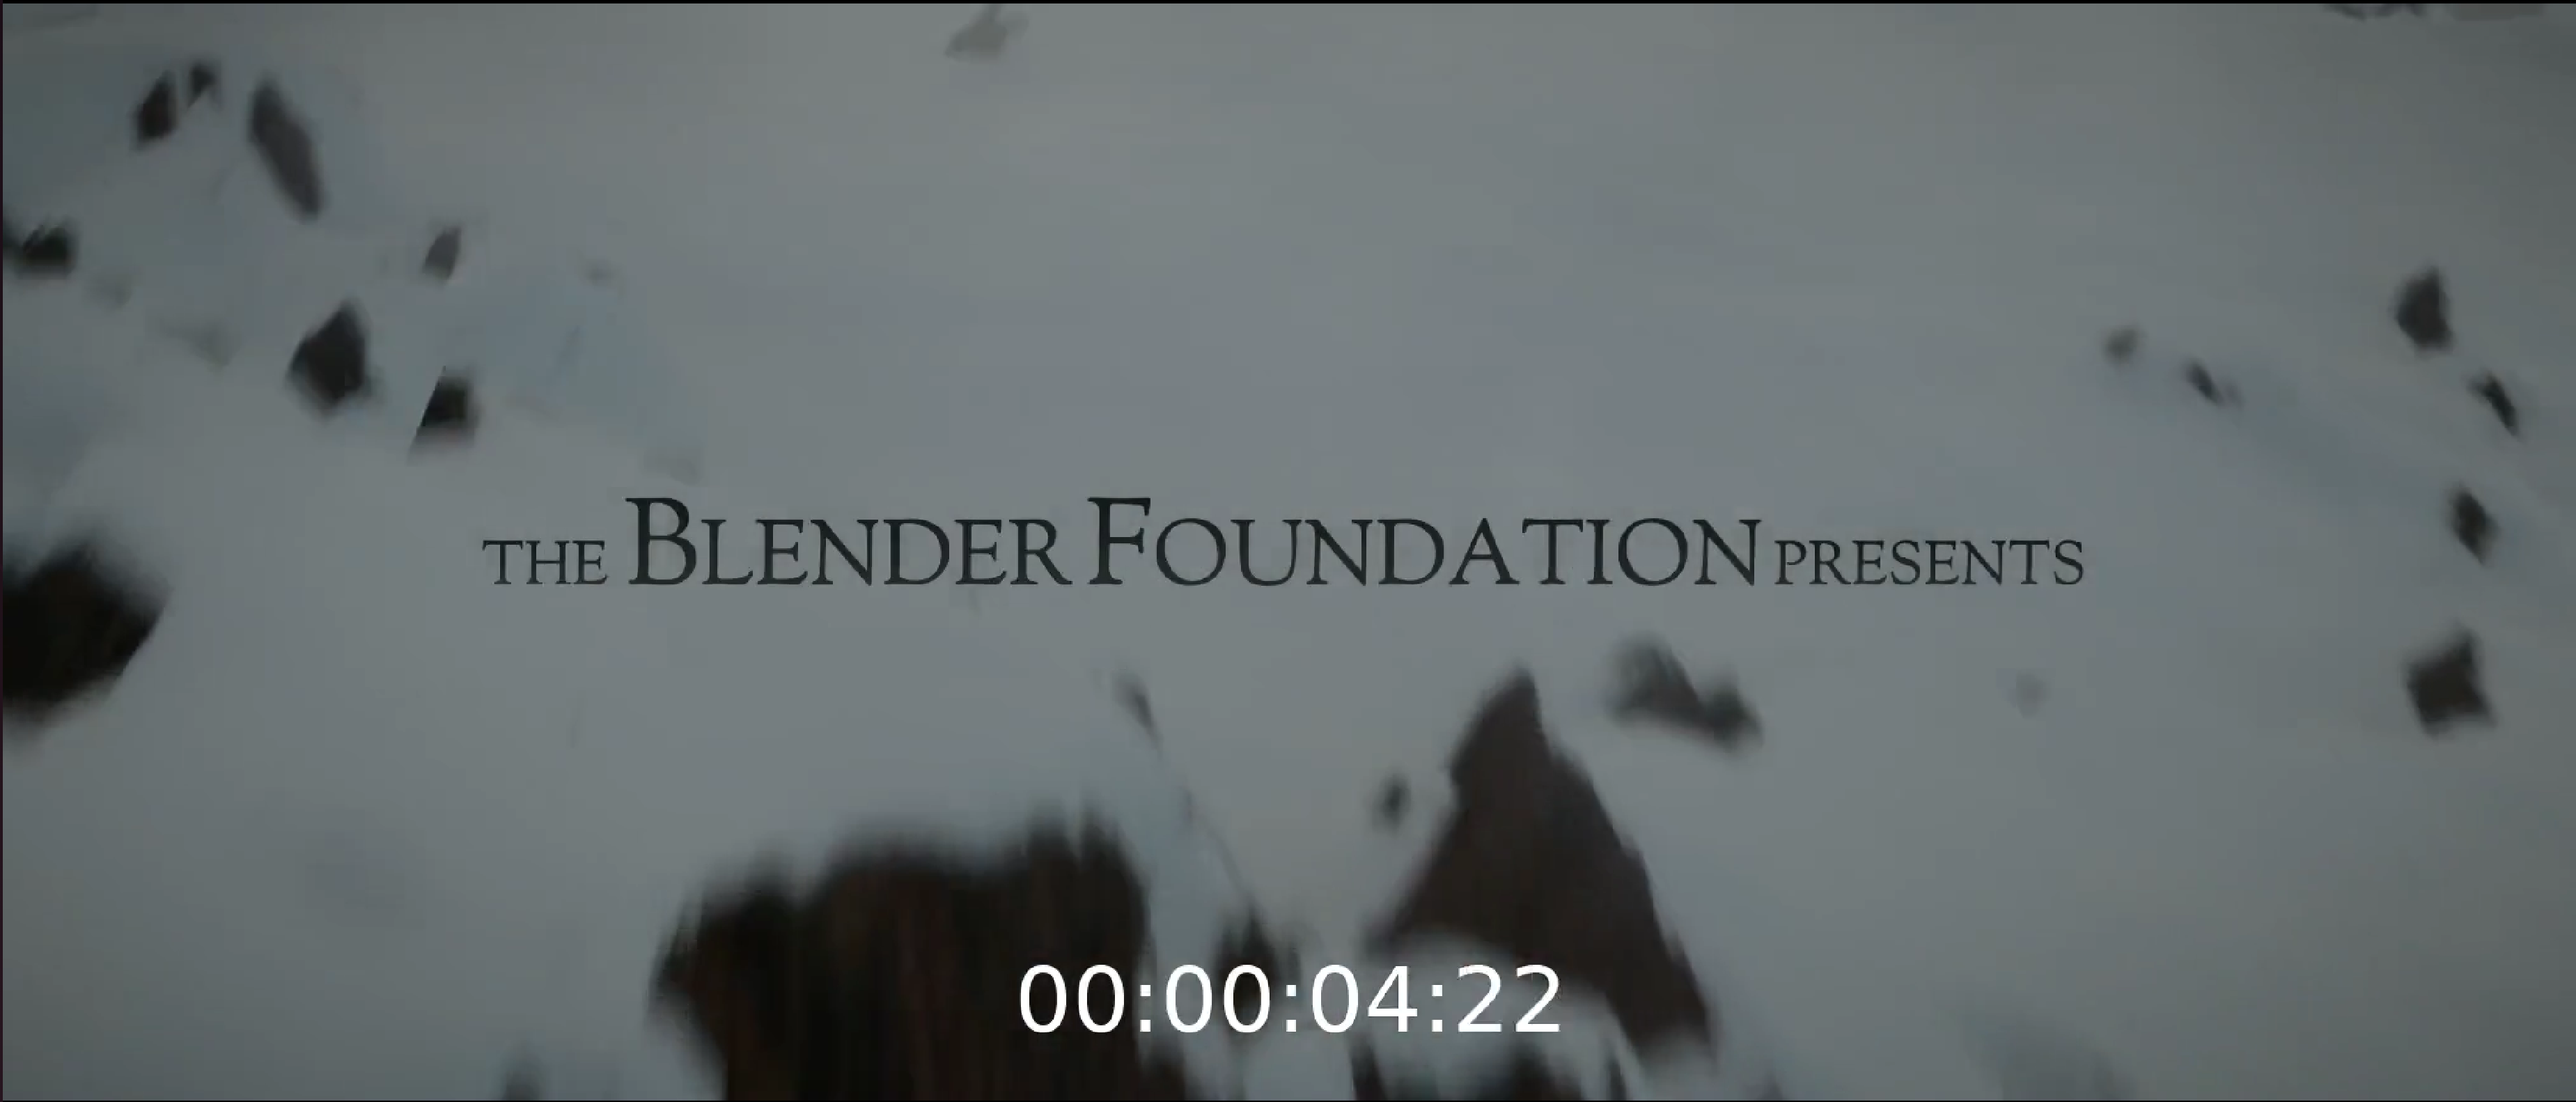
\includegraphics[width=0.9\textwidth]{colourdefault.png}
	Original colours
\end{minipage}\begin{minipage}{0.5\textwidth}
	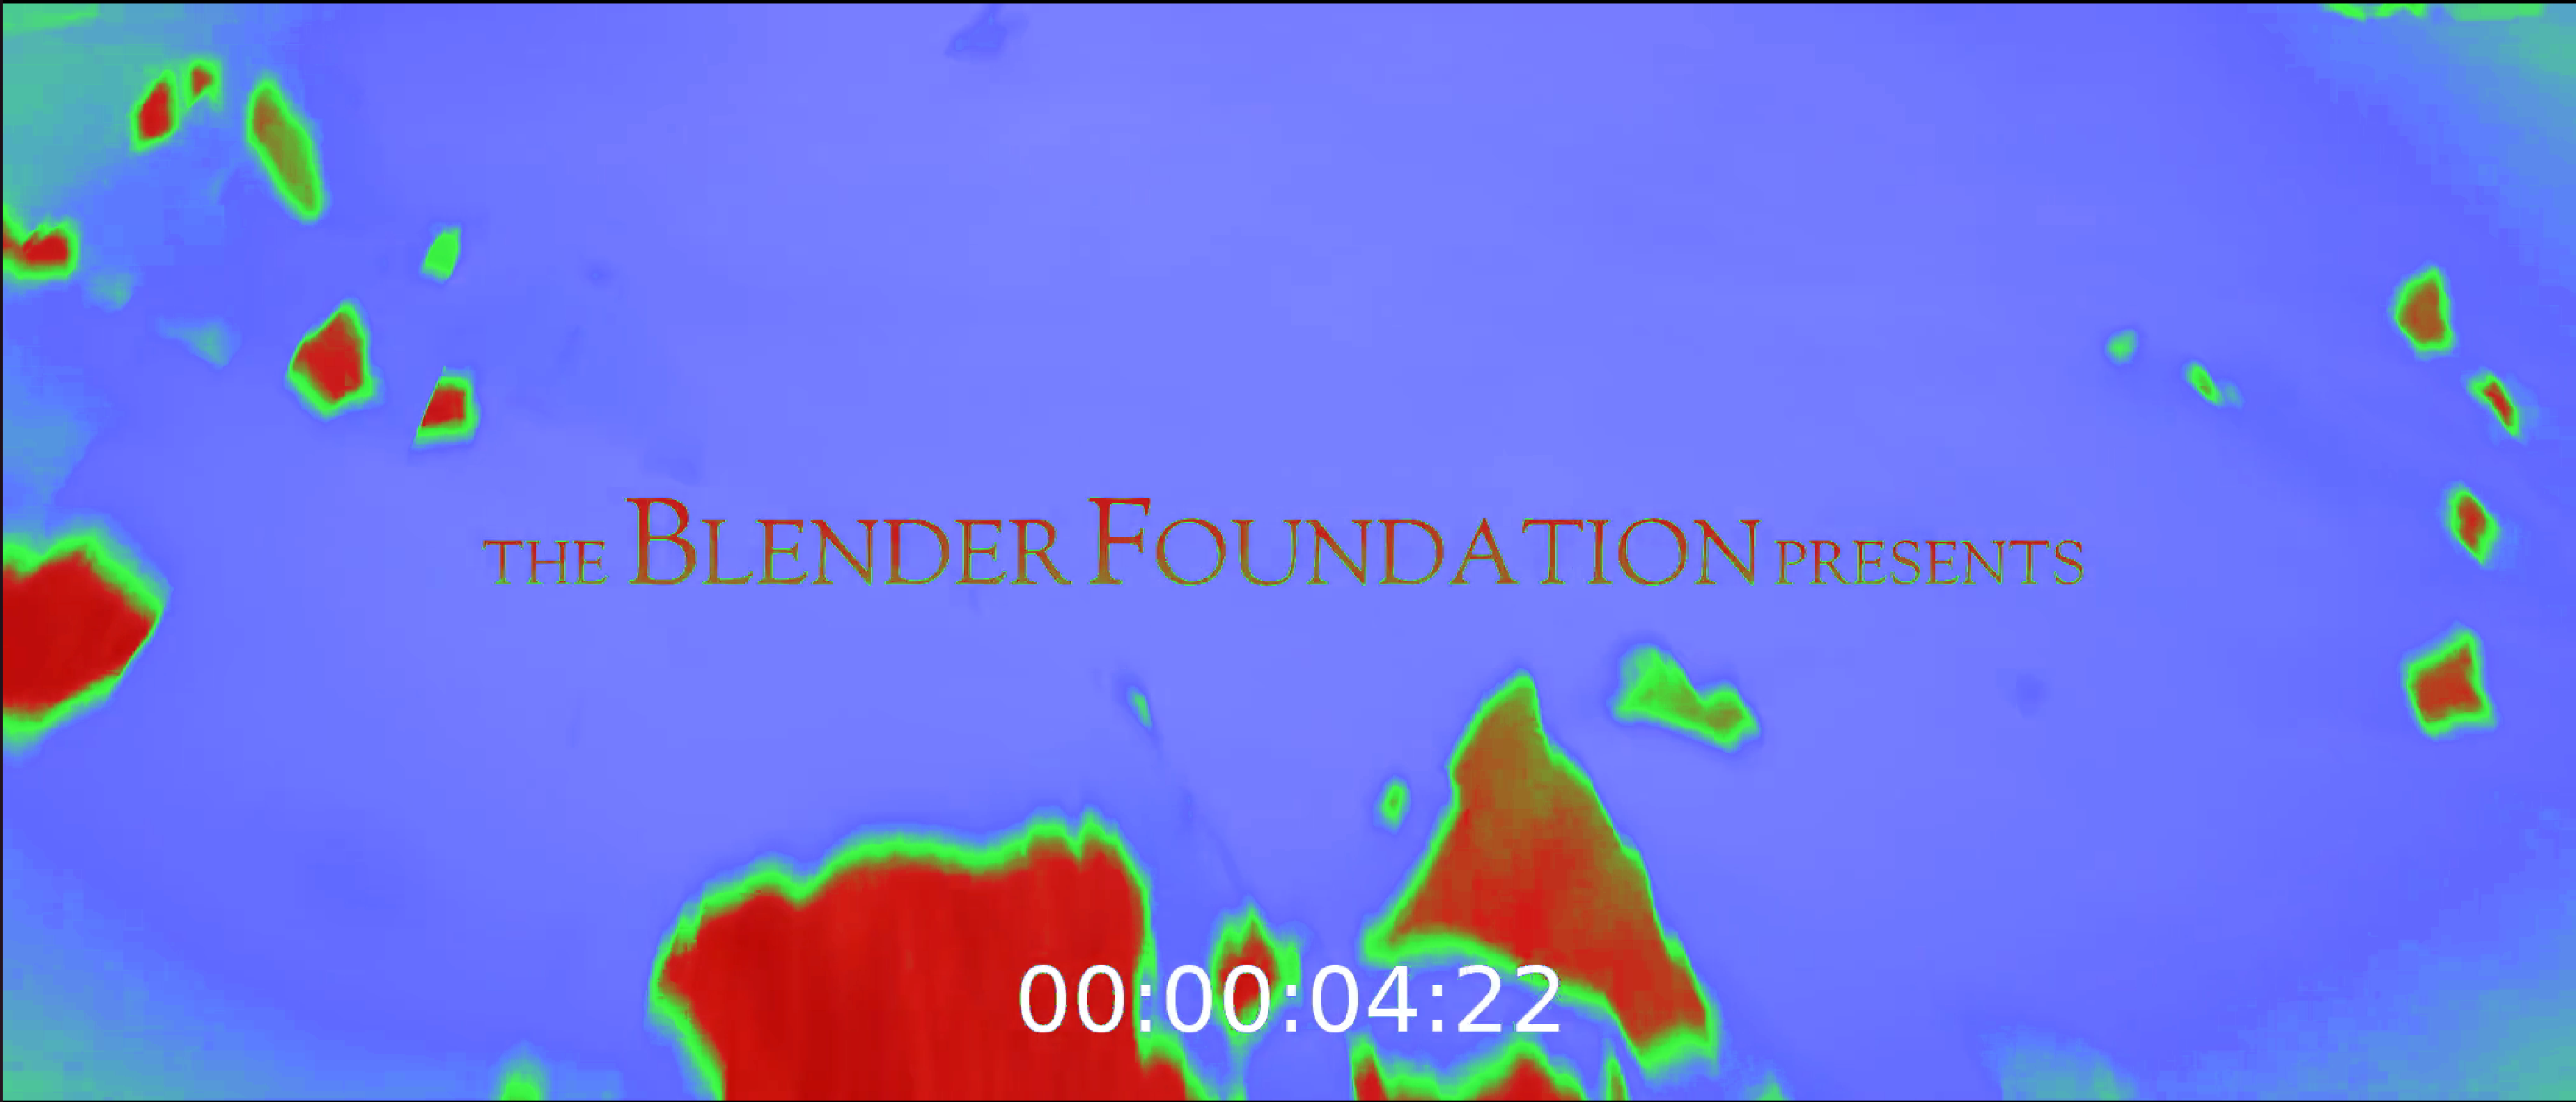
\includegraphics[width=0.9\textwidth]{colourhigh.png}
	Colours with \texttt{av.rs=1} \texttt{av.gm=1} \texttt{av.bh=1}
\end{minipage}

Adding filter to \texttt{local\_melt.py} to execute it in the Accurate Player using JIT:
`
\begin{center}
	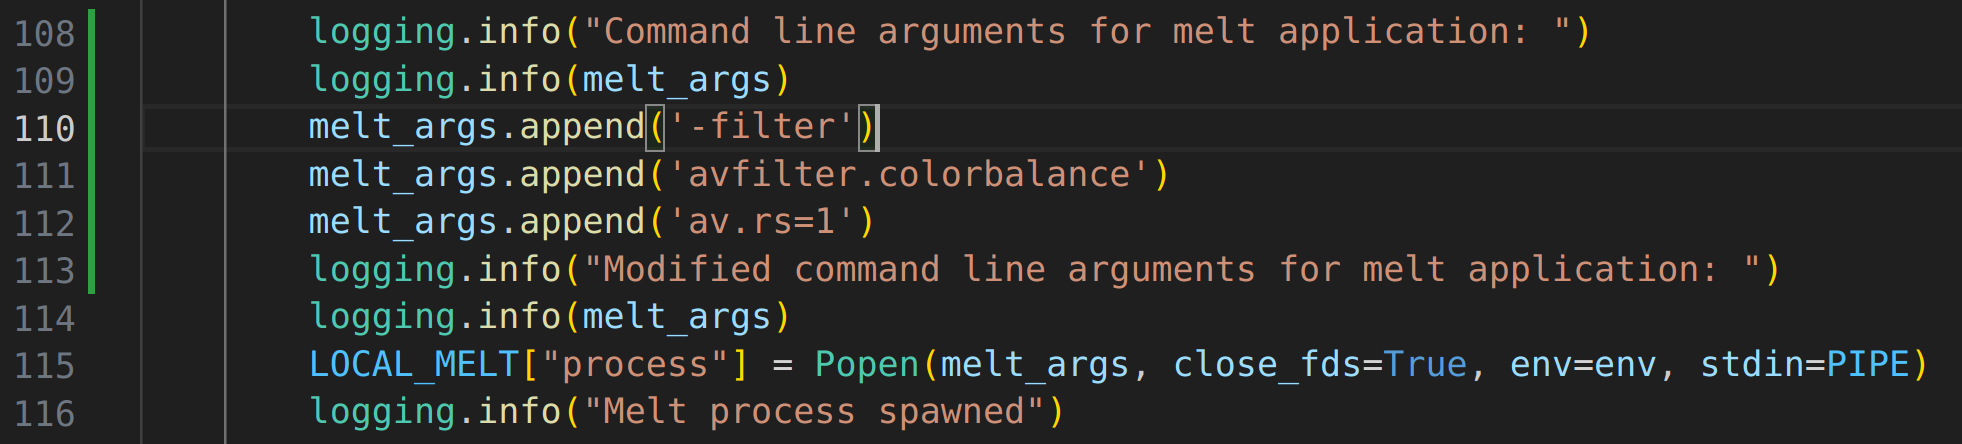
\includegraphics[height=0.13\textwidth]{code.png}
	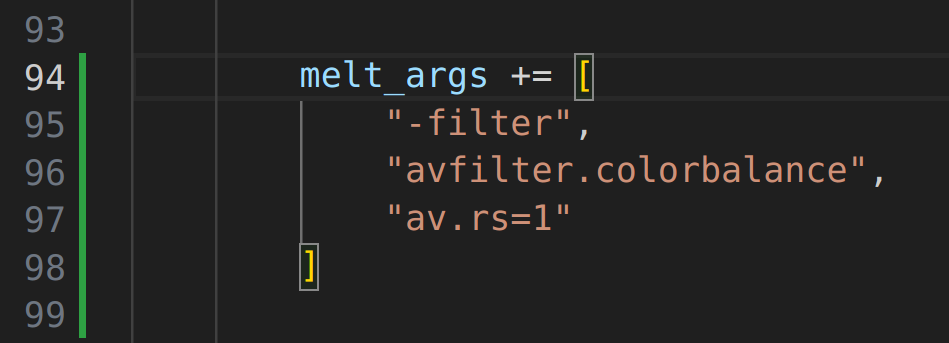
\includegraphics[height=0.13\textwidth]{codecleaner.png}
\end{center}

\begin{center}
	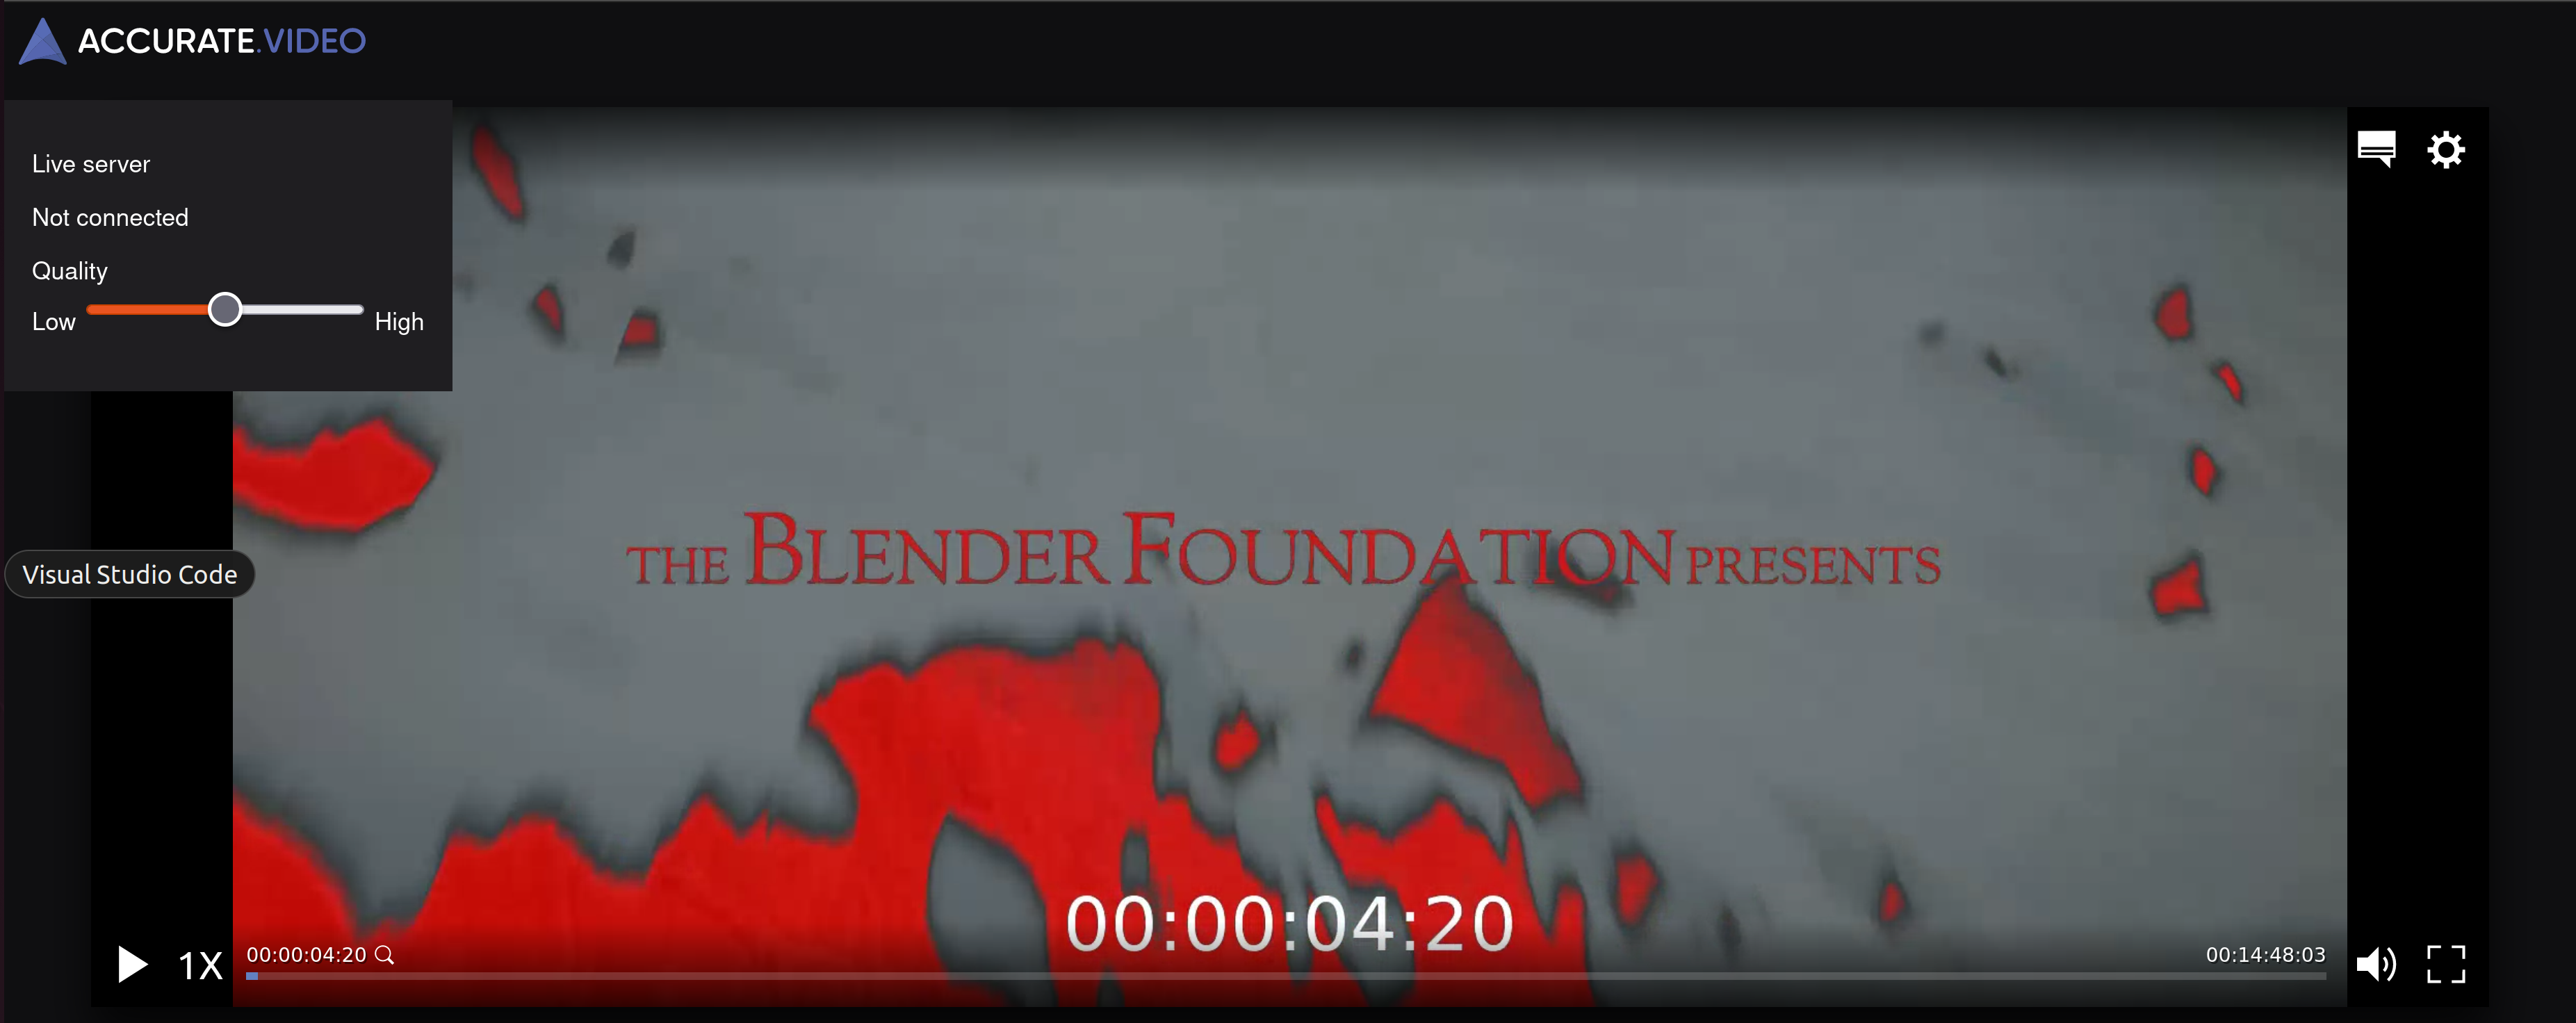
\includegraphics[width=0.8\textwidth]{ap_red.png}
\end{center}













%---------------------------------
\subsubsection{Data flow}

The user initiates a session through the browser, which then initiates the \texttt{main.py} script.
Control commands are then sent from the browser to \texttt{main.py} with a WebRTC data channel.

From the \texttt{main.py}, the control commands get sent to Melt via \texttt{stdout} (standard output) and \texttt{stdin} (standard input). These are the default input and output channels, that allow the Python script communication with other components.
Data written to \texttt{stdout} by the Python code can be captured or redirected and data from an external source can be read from \texttt{stdin} by the Python script. \cite{python}

\begin{figure}[H]
	\centering
	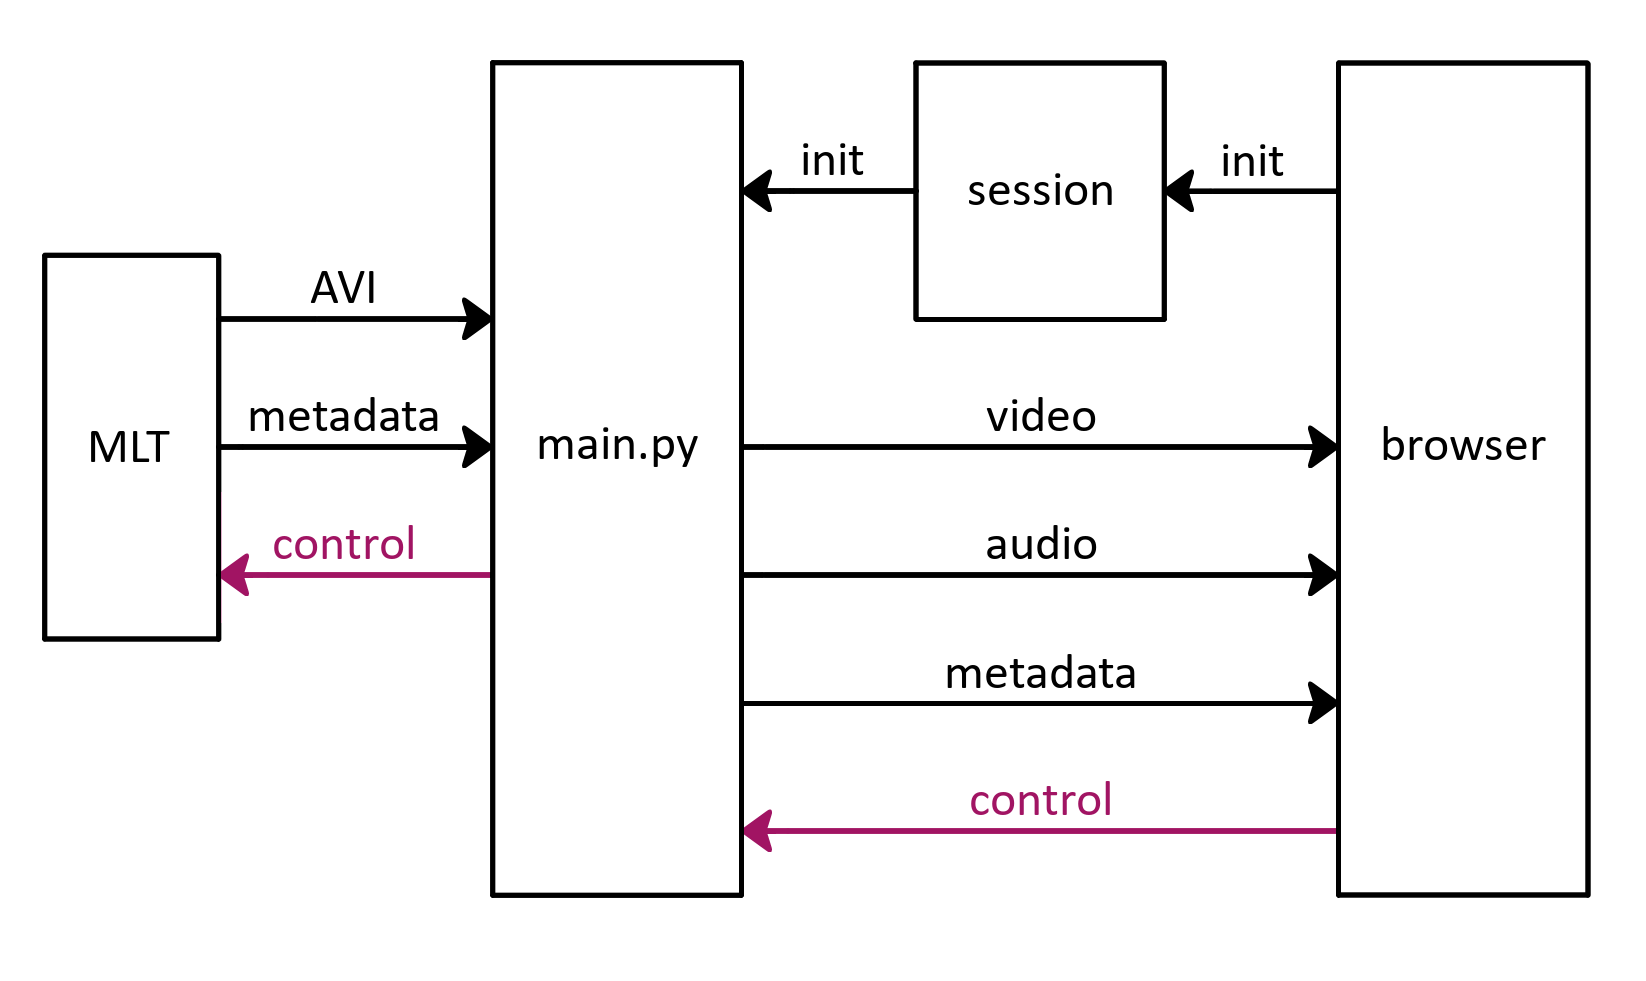
\includegraphics[width=0.5\textwidth]{IM_control.png}
	\caption{Control commands in the system architecture}
	
\end{figure}


Melt sends an AVI stream with the rendered video and audio to the \texttt{main.py} via a named pipe and status messages and metadata via another named pipe.
AVI is a file format that can contain audio and video information to allow synchronized playback of audio and video components.~\cite{avi} AVI was further described in Section~\ref{subsection:technicalbackground} and named pipes in Section~\ref{subsection:technicalbackground}.

\begin{figure}[H]
	\centering
	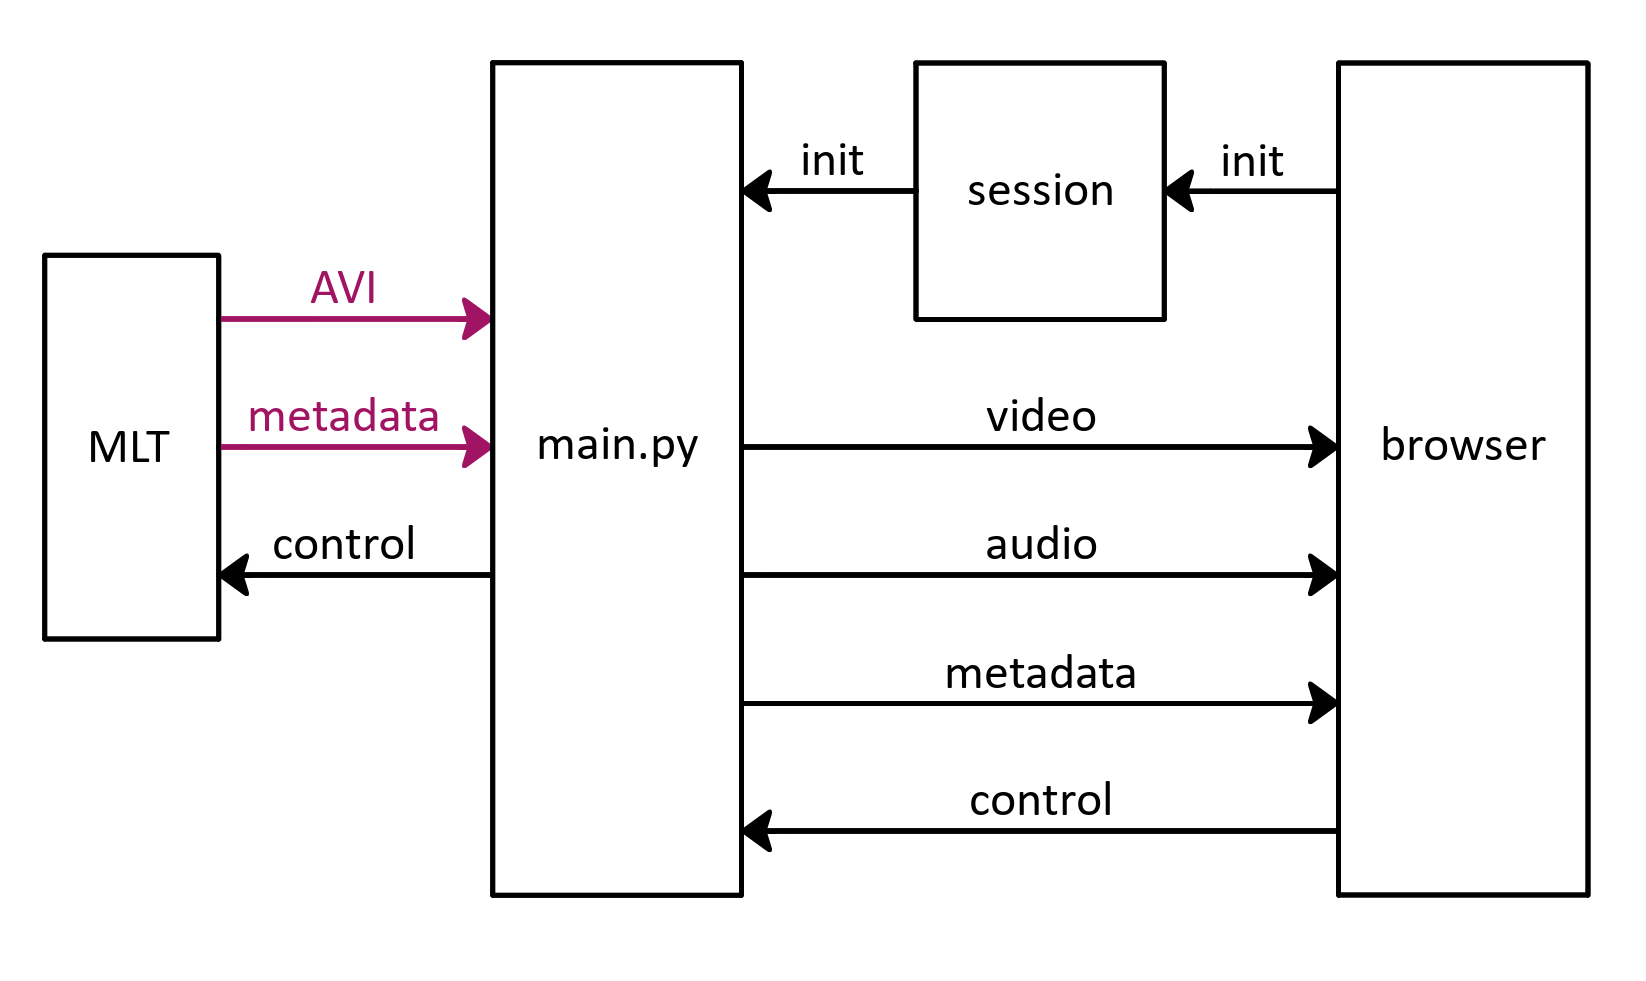
\includegraphics[width=0.5\textwidth]{IM_avi.png}
	\caption{AVI stream in the system architecture}
\end{figure}


Then the audio and video from the incoming AVI stream is extracted by the \texttt{main.py} script to then encode it for sending it to the browser with WebRTC. The WebRTC connection serves as a direct communication channel between the browser and the backend, enabling real-time data exchange, involving audio, video, or other data streams. 

TODO: Is is encoded into h-264 here?

%It has the ability to extract specific channels from the rendered audio, to %be rendered to an stereo stream for WebRTC.
%It does not appear to be possible to encode surround sound for WebRTC, despite WebRTC using the Opus codec which is surround capable.
%This may be a limitation in `aiortc`, in WebRTC or in the browser, or all three.
%

\begin{figure}[H]
	\centering
	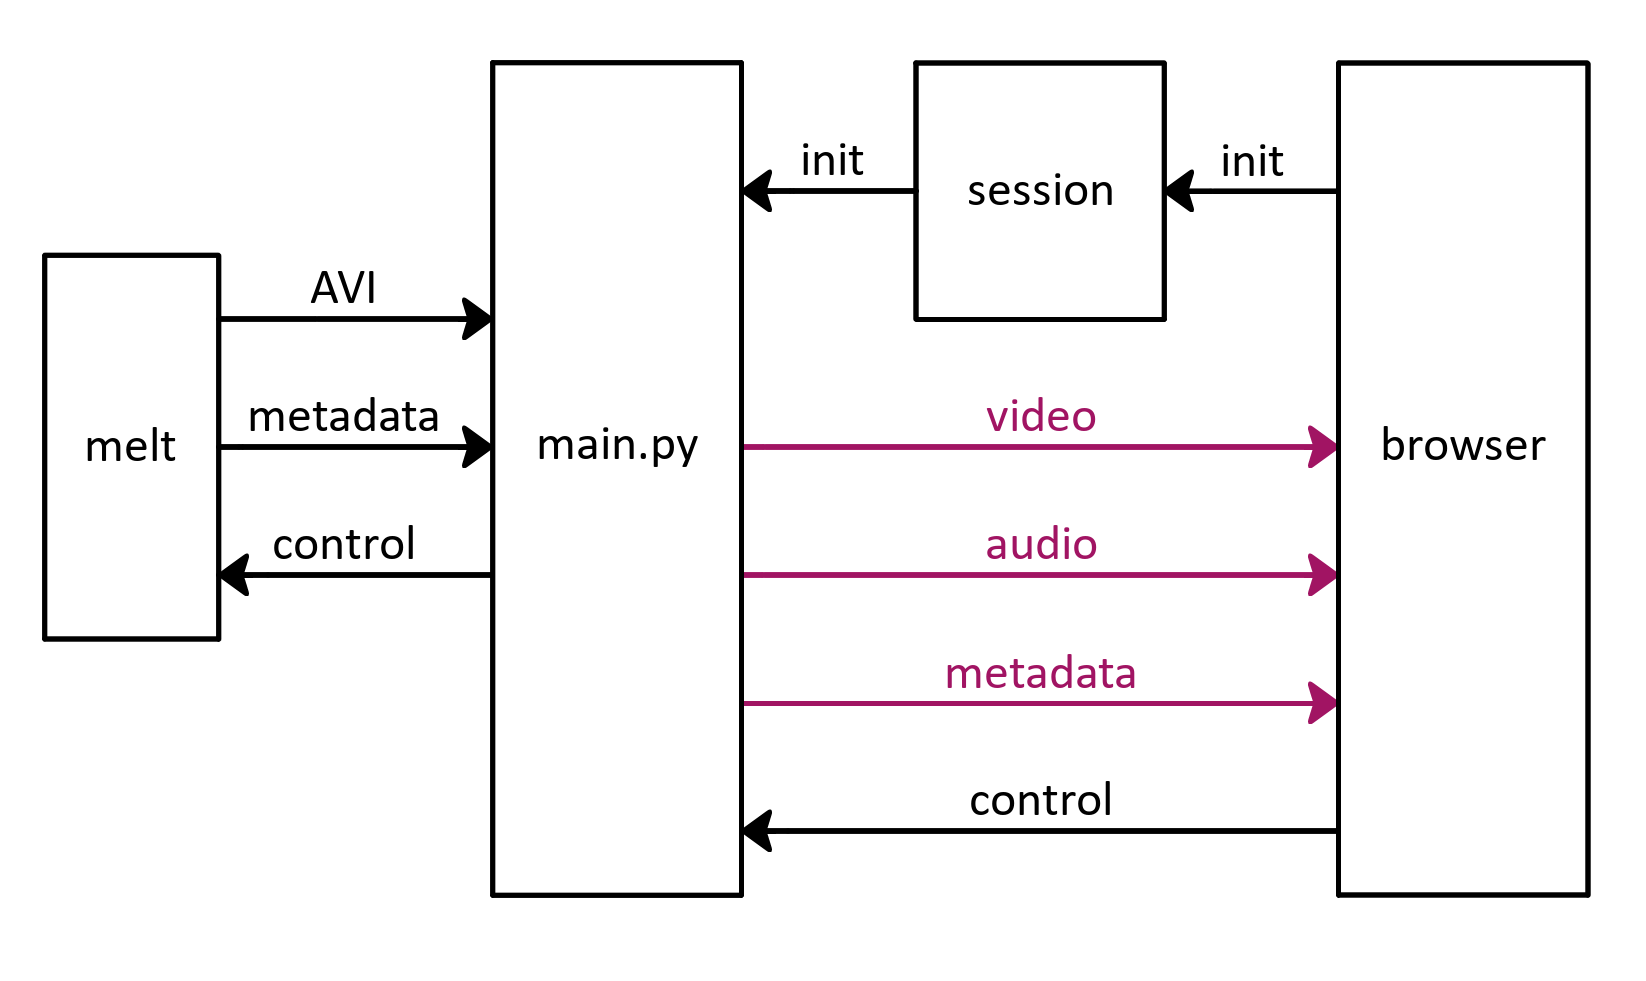
\includegraphics[width=0.5\textwidth]{IM_wrtc.png}
	\caption{WebRTC connection in the system architecture}
\end{figure}

Then the JavaScript client of the browser receives the video and audio and plays it. In addition to this, it
receives metadata from the \texttt{main.py} script and sends commands and ping responses over the control channel.


\begin{figure}[H]
	\centering
	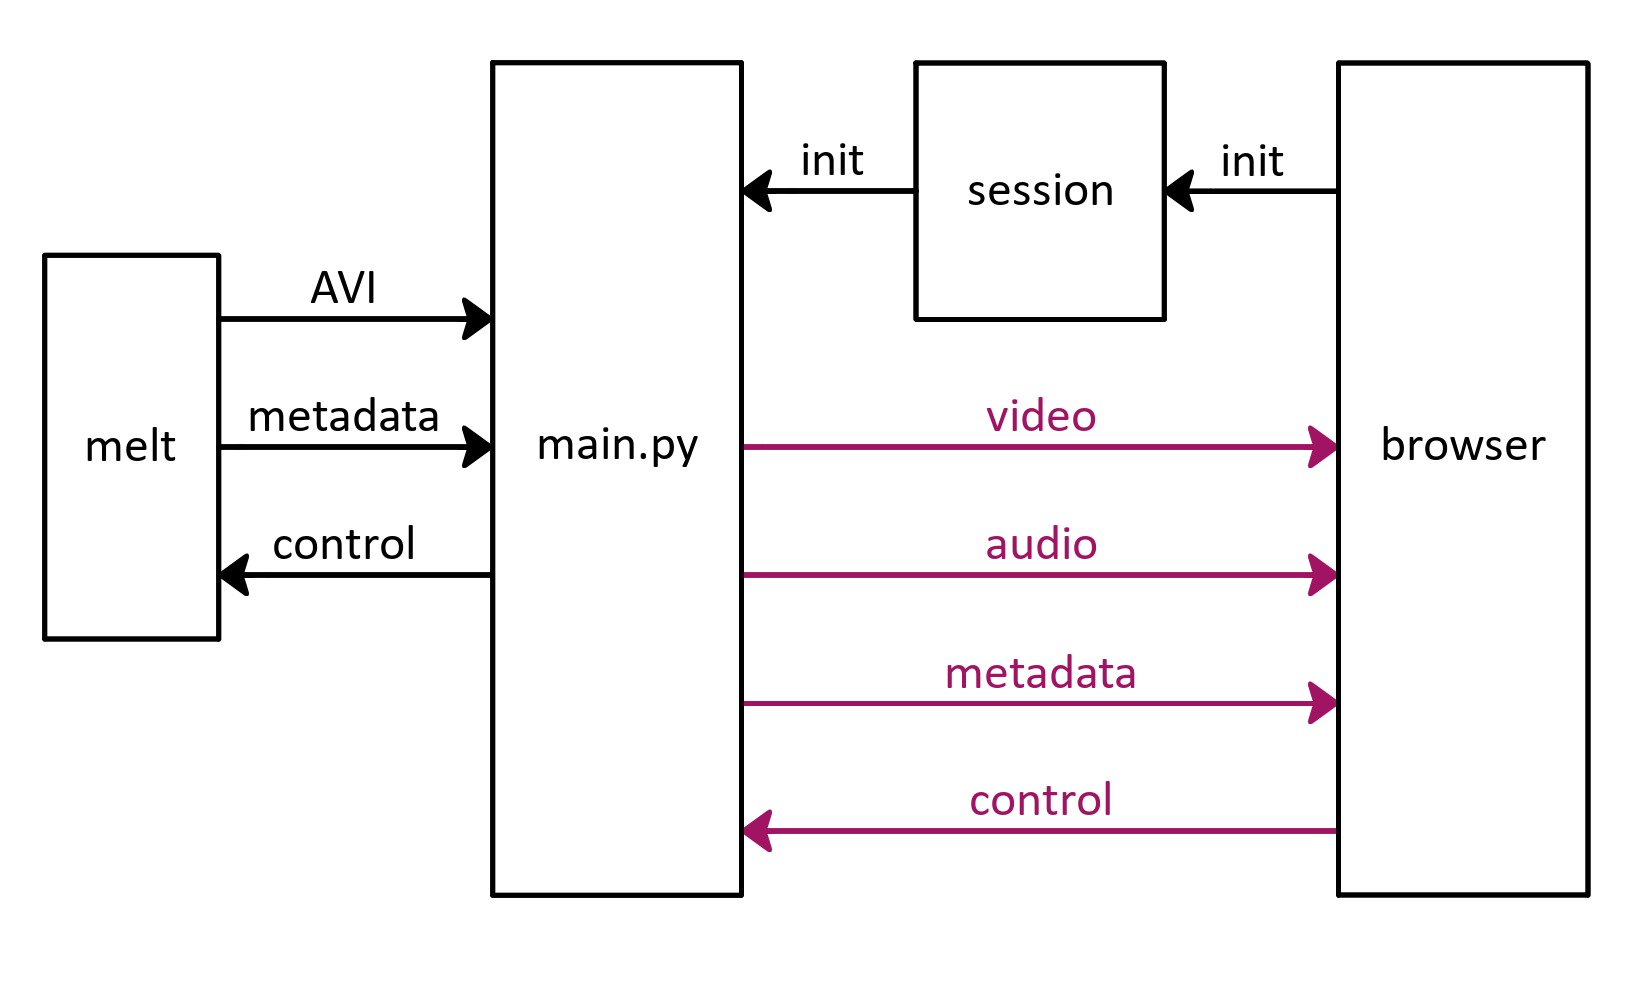
\includegraphics[width=0.5\textwidth]{IM_wrtc_control.png}
	\caption[WebRTC and control in the system architecture]{WebRTC connection and control commands in the system architecture}
\end{figure}

Melt and the \texttt{main.py} script are started once for each JIT session with a parameter that presents the media from the start on.

%`main.py` and `melt` is started once for each JIT session, and media is presented to it on startup. 

\subsubsection{Session}

\texttt{Session} is a java-based service, designed to support machine-to-machine interaction between the browser and the backend (\texttt{main.py} and Melt). Web services allow different applications, that often run on different platforms and are written in different programming languages, to communicate with each other.~\cite{webservice}

The \texttt{Session} service exposes a REST API (described in Section~\ref{subsection:technicalbackground}) for initiating a JIT session with specified media details. 

% Additionally, it leverages AWS, specifically utilizing the Auto Scaling Group (ASG) feature to manage a cluster of instances dynamically, ensuring scalability and efficient distribution of JIT sessions across the instances in the cluster.

% AWS
%2. **AWS (Amazon Web Services):**
%- **Definition:** AWS is a cloud computing platform provided by Amazon. It offers a wide range of services, including computing power, storage, databases, machine learning, and more, allowing businesses to scale and grow without the need for significant upfront investments in physical infrastructure.

% ASG cluster
%3. **ASG Cluster (Auto Scaling Group):**
%- **Definition:** An Auto Scaling Group is an AWS service that automatically adjusts the number of compute instances (e.g., virtual machines) in response to changes in demand or other specified conditions. It helps ensure that the desired number of instances are available to handle varying workloads.



%`session` is a Java-based service that presents a REST api that can be used to start a new JIT session given a description of the media to use. It also has support for managing a full ASG cluster on AWS, and distribute new JIT sessions on the instances in 
%the ASG.
%
%For more information on each component see:
%* [`melt`](https://github.com/sirf/mlt.git)
%* [`main.py`](jit/README.md)
%* [`session`](session/README.md)
%

For development and quick testing without the session service, JIT can be started in a Docker container. A Docker container is in isolated environment in which an application can be run and Docker is the platform that enables the usage of those containers.~\cite{docker}


\begin{figure}[H]
	\centering
	
\includegraphics[width=0.6\textwidth]{IM2.png}
	\caption{System architecture when run in a docker container.}
\end{figure}


%## Development
%
%For development and quick testing without the session service, on can either start JIT as a docker, or run JIT directly on your computer. The latter has some problems if you're on an Apple ARM.
%
%Run the docker:
%
%`docker/main/main.sh --threads 16 --port 8080 $VIDEOFILE`
%
%Where `$VIDEOFILE` is either a local path or a URL. `threads` and `port` are both optional, with current default values set to 72 threads and port 8080.
%
%To run JIT directly, see [`jit/README.md`](jit/README.md).
%
%### Open Docker IPs
%
%Your Docker container will get an IP in the style of 172.17.0.\*. Using e.g. Docker CE on Linux this IP will be reachable from outside the container. However, on Docker Desktop for Mac, this IP will not be opened. This will cause problems. There is a service that can fix this. You **install and activate it once** by doing this:
%
%```
%# Install via Homebrew
%brew install chipmk/tap/docker-mac-net-connect
%
%# Run the service and register it to launch at boot
%sudo brew services start chipmk/tap/docker-mac-net-connect
%```
%
%
%## Deployment
%
%Currently the only way supported for deployment is by using EC2 instances on AWS. An AMI is created by CI on release, containing a 
%local instance of the `session-service`, together with `main.py`, `melt` and anything else needed to start JIT processes on the EC2 
%instance. For more information about what the AMI contains, and how configuration can be fed to it see [`ami/README.md`](ami/README.md).
%
%### Terraform
%
%Terraform modules are supplied that simplify setup of either single EC2 instances or a full ASG cluster of instances, including 
%`session-service` running as an orchestrator on ECS. See [`terraform/README.md`](terraform/README.md) for more information on 
%available modules, their parameters and outputs.
%






%-------------------------------------------------------------------------------------------------------
\subsection{Technology} \label{subsection:technology}
% Discuss the technologies and tools chosen for the implementation.








	
	
	
\end{document}